\documentclass{article}
\usepackage{listings}
\usepackage{amsmath}
\usepackage{graphicx}

\begin{document}

\title{MAT362 - Project2 Report}
\author{Christopher D. Whitney}

\maketitle

\section*{Introduction}
The goals of this project are (1) implement and test multiple tridiagonal solvers, (2) apply them to a cubic spline, (3) to experiment with these solvers to discretize the second derivative operator matrix and finally to approximate the eigenvalues of the second derivative matrix and compare them to exact values. 

\section*{Overview of Algorithms}
In the following section we will outline and describe the algorithms used to implemented this project. 

\subsection*{Direct Method to Solve Trigonal Systems}
The first algorithm implemented for this project is a direct approach to solve tridiagonal systems using Gaussian elimination. It works by the first zeroing out lower diagonal. This is accomplished by iterating over the diagonal matrix and modifying the main and upper diagonal such that the lower will be zero. We do not actually need to change the lower, instead we just treat it as if it has been zeroed out. The second step is start to solve for the $x$'s this is accomplished by first solving for $x_n$ then threw back substitution solve the reset. This algorithm is know as a direct method because it it has a finite number of step unlike an iterative method which will be discussed in the next section. 

\subsection*{Iterative Method to Solve Trigonal Systems}
The second algorithm that was implemented for this project for the tridiagonal solver known as the Gauss Seidel which iteratively updates values of $x$ until a stoping criteria is meet. It updates the new $x$ based on some initial guess usually zero, the lower diagonal, the $b$ matrix and the lower matrix. The iterative formula goes as follows, 

$$ x_{i+1} = \frac{b - U*x_i}{L_i}$$ 

Where $x_i$ is the current $x$ value $b$ is the matrix containing the right hand sides of the system, $U$ is the upper diagonal, $L$ is the lower diagonal and $x_{i+1}$ is the next $x$ value. 

The algorithm terminates when a certain amount of iterations has been met or when the $x_i$ and $x_{i+1}$ are with a tolerance of each-other. 

\subsection*{Construction of a Cubic Spline}
A cubic spline is a piece wises cubic function that fits a given set of data over a set of intervals and has the following form, 
$$ S_j (x)=a_j +b_j(x-x_j)+c_j(x-x_j)^2 +d_j(x-x_j)^3$$

The cubic spline construction algorithm thus solves for each one of these constants for each on the intervals. 

\section*{Problem 1}

\subsection*{Part A}
After implementing the direct method of trigonal solver using the algorithm described above we tested it on two systems. One is a much smaller system and the second is a little bit larger. In both cases the systems exact solutions were known. The following is the results. \\

\textbf{System 1}\\  
$$ x + y = 3 $$  
$$ 2x+y = 4 $$ 
Where the exact solutions are $x=1$ and $y=1$. After running the solver to approximate the solutions we also obtained $x=1$ and $y=1$. We can see with this system the solver is able to calculate the exact solution.  \\

\textbf{System 2}\\
$$ x + y = 4$$ 
$$ x+y+z=3$$ 
$$y+z=2$$
Where the one possible exact solution is $x=1$, $y=3$, and $z=-1$. Using the direct method we obtain the approximations of 
 $x=4$,$y=-3$,$z=2$ which are solutions to the system however the are not the exact same as our original solutions. We can see that $y$ has a sign difference and $x$ and $z$ are completely different. 

\subsection*{Part B}
For this section of the project we implemented an arbitrary larger tridiagonal system and used the built in MatLab operation $mldivide$ to solve the system. We determined threw online MatLab documentation that if the matrix is square, sprases and triangular then the MatLab operation uses the diagonal solver. Since, are system fits both those criteria we believe the operation used that algorithm.  

\section*{Problem 2}
For this section of the project we implement the Gauss Sidel solver which is an iterative solve described above and used it to solve same system as in problem 1 part a. For the first system the method was unable to come up a solution that was a small numbers, and for the second system the algorithm was able to come up with an exact solution. One can run source code for exact values. 

\section*{Problem 3}
After implementing the cubic spline constructor which uses a traditional solver we tested the algorithm on two data sets, the first is a arbitrary curve and the second is the duck picture from the course text.  

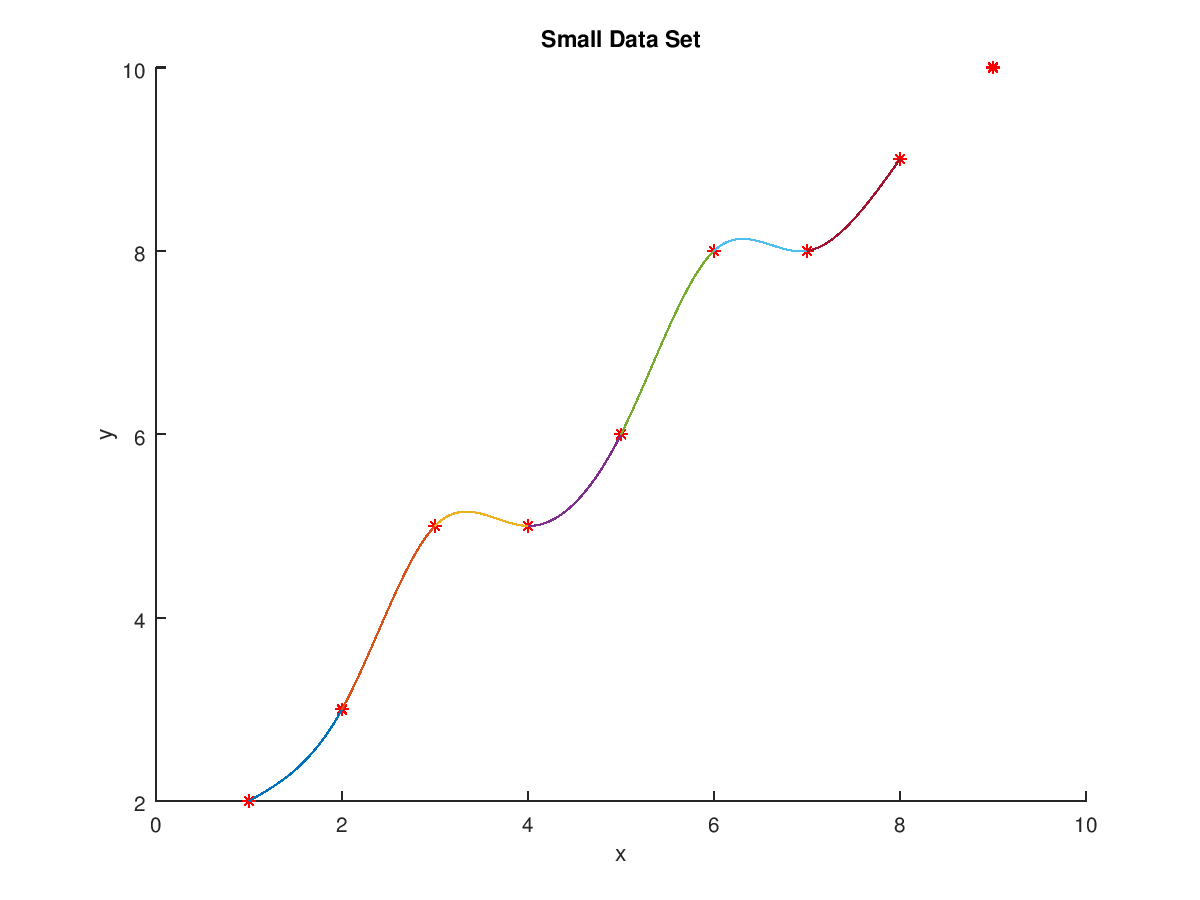
\includegraphics[height=8cm]{problem3a.png}\\
Figure: Cubic spline for an arbitrary curve.

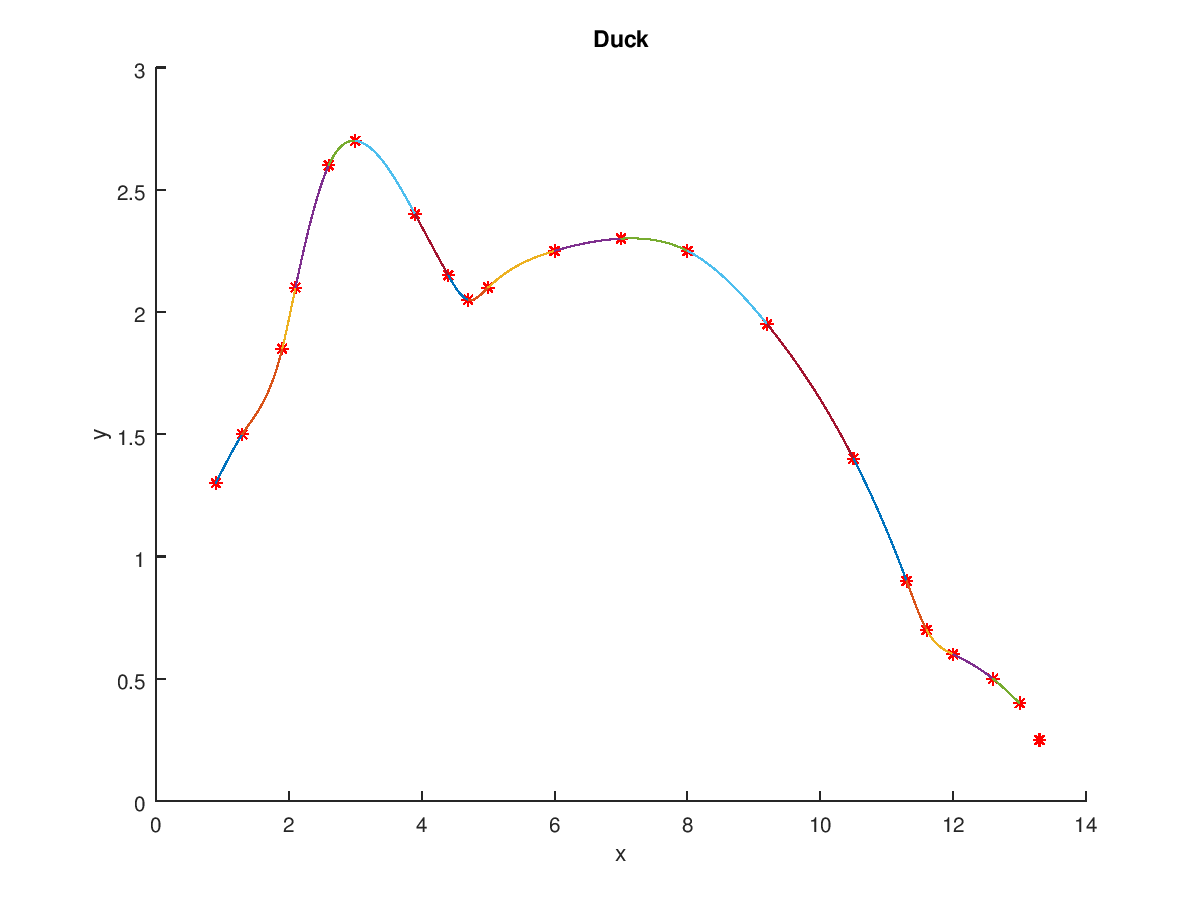
\includegraphics[height=8cm]{problem3b.png}\\
Figure: Cubic spline for a duck image.

\section*{Problem 4}

\subsection*{Part A}
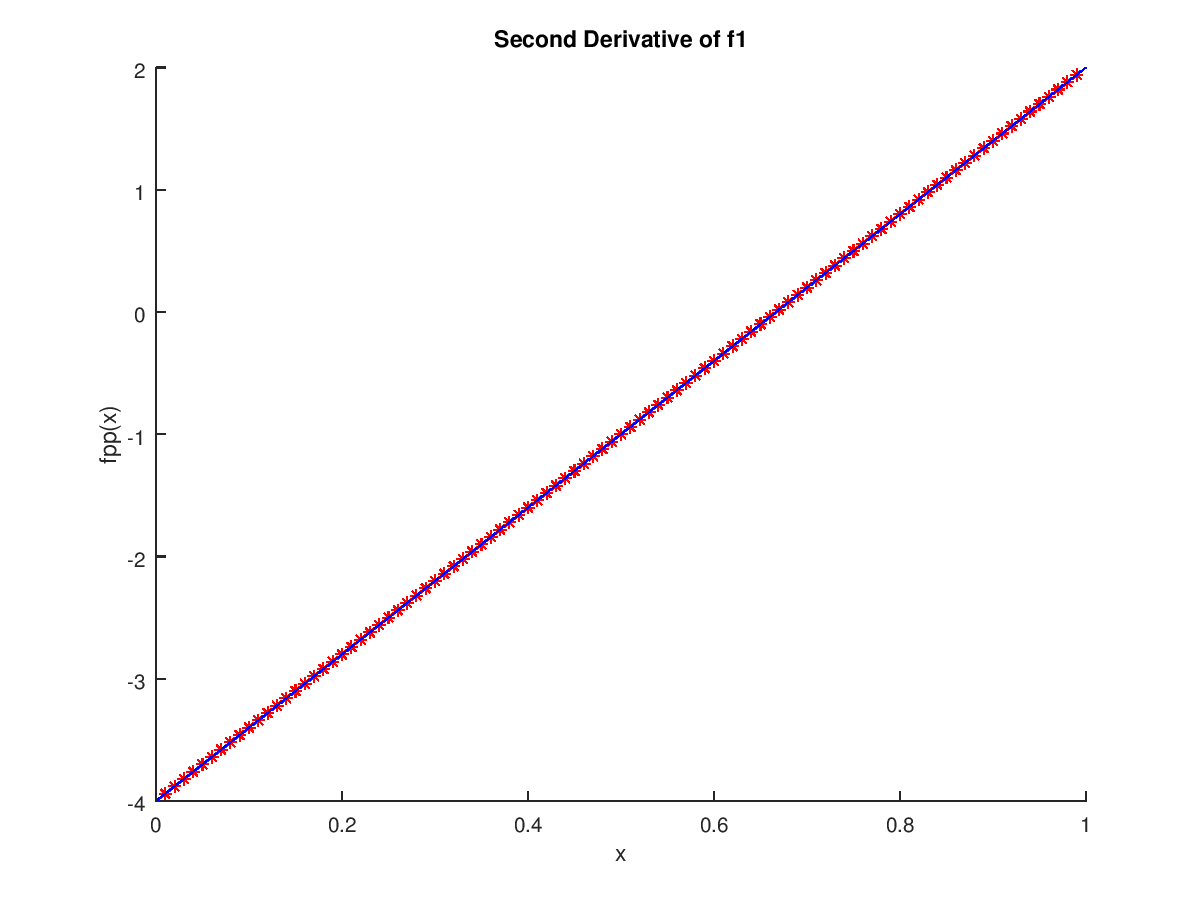
\includegraphics[height=8cm]{problem4a.png}\\
Figure: The red stars the approximations and the blue lines are the exact solution. 

$$\begin{tabular}{l | l | l } 
	\hline
	x & Actual & Approximation \\
	\hline
	0.1 &  -3.4 & -3.4  \\
	0.2 & -2.8 & -2.8 \\
	0.3 & -2.2 & -2.2\\
	\vdots & \vdots & \vdots \\
	0.99 & 1.94 & 1.94\\
\end{tabular}$$


\subsection*{Part B}
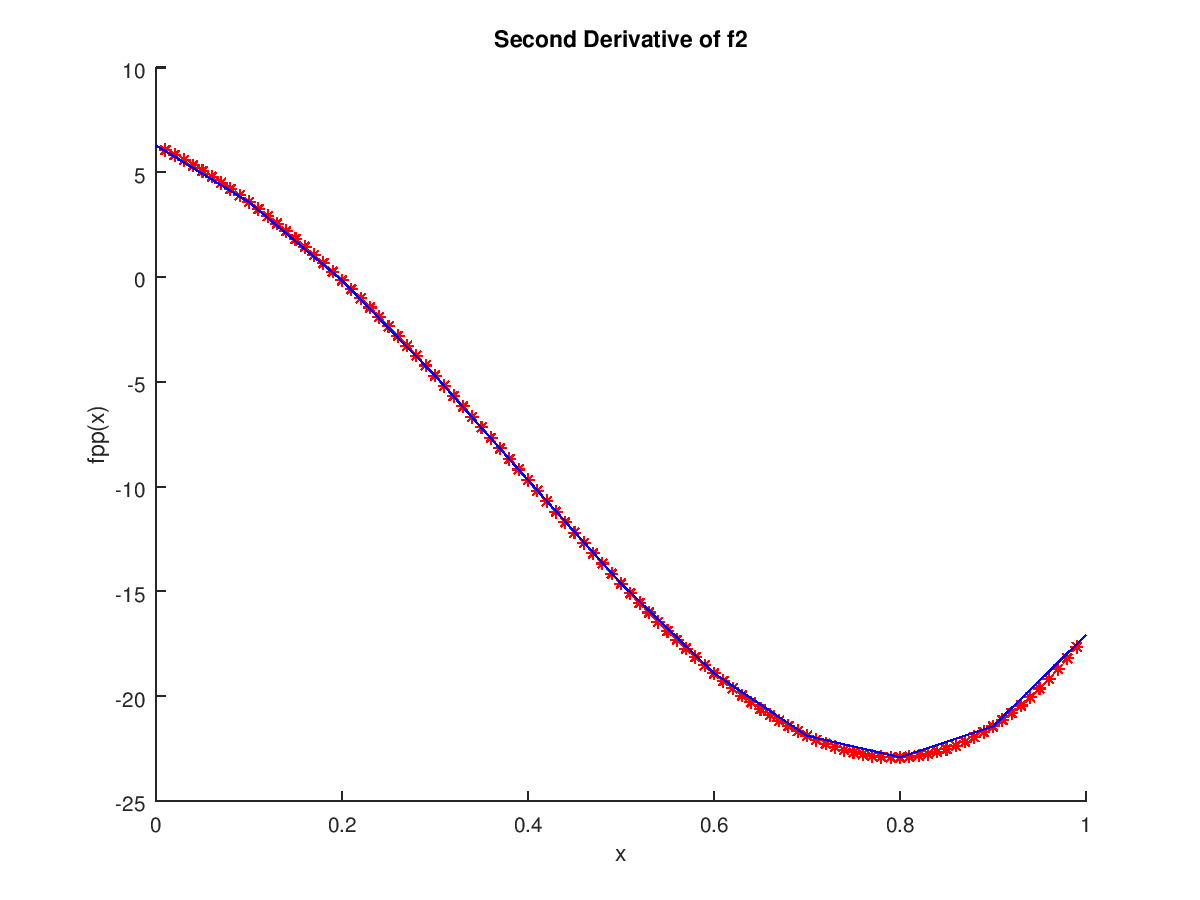
\includegraphics[height=8cm]{problem4b.png}\\
Figure: The red stars the approximations and the blue lines are the exact solution. 

$$\begin{tabular}{l | l | l } 
	\hline
	x & Actual & Approximation \\
	\hline
	0.1 &  3.5750 & 3.574149 \\
	0.2 & -0.15905 & -0.159733 \\
	0.3 & -4.7009 & -4.701260 \\
	\vdots & \vdots & \vdots \\
	0.99 & -17.651 & -17.648436\\
\end{tabular}$$


\subsection*{Part C}
From the three-point midpoint formula in the course text we know the error term is, 
$$ R(x) = \frac{-h^2}{f^{(3)}(\epsilon_0 )} $$

\textbf{a}
Since the actual second derivative increases to infinity as x goes to positive and negative infinity, we shall choose the bounds as the upper limit on the graphed function, 1. 
$$ R(x) \leq \frac{-(0.01)^2}{-2} = 5*10^{-5}$$

\textbf{b}
By investigating the actual second derivative we can observed that a maximum for the function is 60, thus we bound the error by this value. 

$$ R(x) \leq \frac{-(0.01)^2}{f^{(3)}(60 )} $$
$$  \leq \frac{-(0.01)^2}{f^{(3)}(60 )} $$
Where $f^{(3)} = e^xsin(\pi x)-3 \pi^2 e^x sin(\pi x) + \pi^3 (-e^x)cos(\pi x) + 3 \pi e^x cos(\pi x)$\\
$f^{(3)}(60) = 3e^{60} \pi - e^{60} \pi^{60}$
$$  \leq \frac{-(0.01)^2}{ 3e^{60} \pi - e^{60} \pi^{60} } $$

\section*{Problem 5}
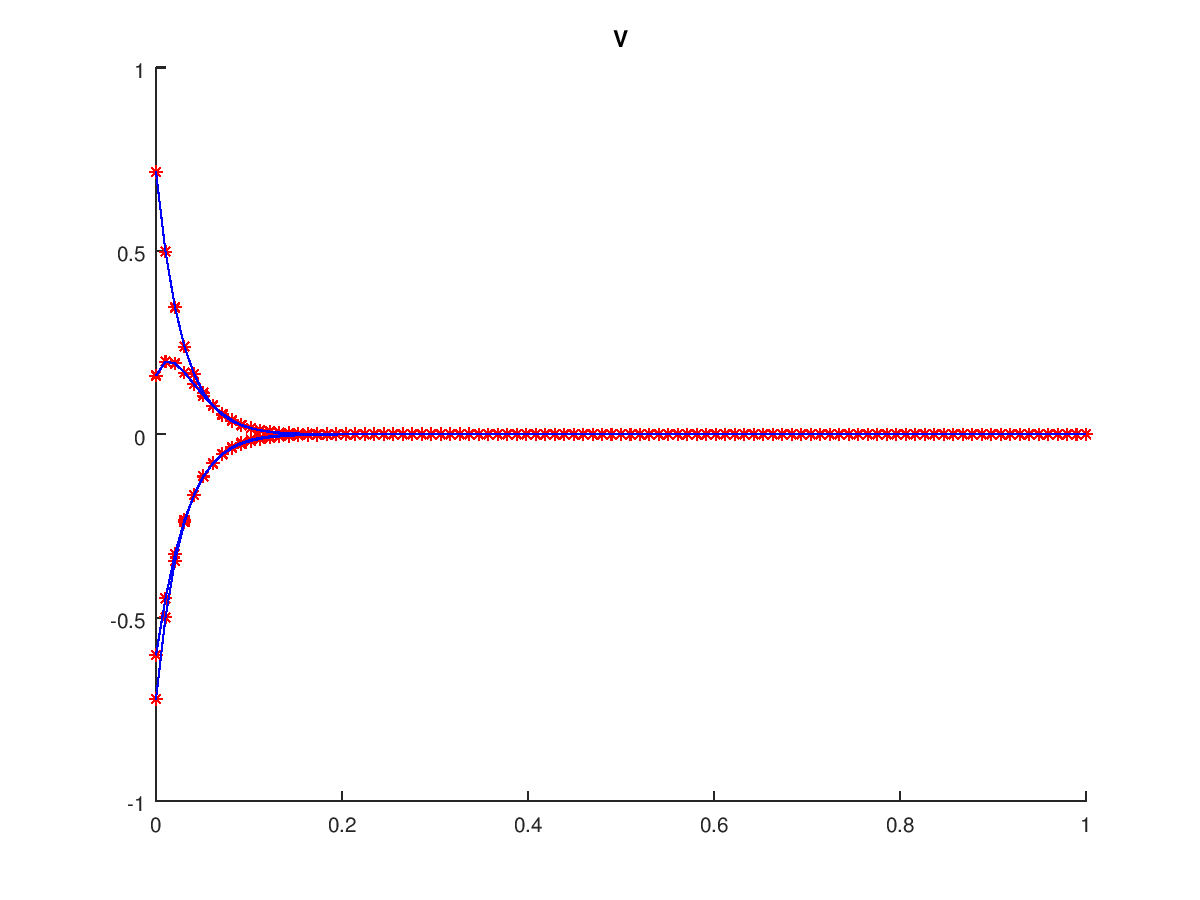
\includegraphics[height=8cm]{problem5.png}\\
Figure: Red stars are approximations and the blue lines are the exact solution. 

\end{document}
